\renewcommand{\labelitemi}{\textbullet}
\begin{itemize}

\item El TAD Pokemon es String porque asumimos que lo \'unico que nos interesa saber es el tipo de pokemon. Asimismo, el TAD Jugador es Nat que se refiere a un ID \'unico. El resto de los detalles relacionados (como sus posiciones, conexi\'on del jugador, etc.) los maneja el TAD Sistema.

\item Para el TAD Mapa el enunciado nos pide saber las posiciones v\'alidas y como est\'an conectadas entre s\'i, y para esto \'ultimo supusimos que, adem\'as de saber si dos puntos est\'an conectados, nos interesa saber si existe una conexi\'on directa entre ellos (es decir, si hay un camino entre ambos sin otras posiciones en el medio)

Por ejemplo, los siguientes casos se consideran distintos mapas (los puntos son posiciones y las l\'ineas son conexiones directas):

\bigskip
\centerline{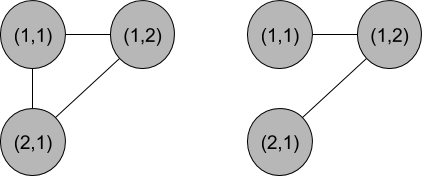
\includegraphics[scale=0.5]{nodos-mapa.png}}

Cabe destacar que esto no afecta la l\'ogica del juego, ya que los requisitos para movimientos v\'alidos siguen siendo 1) una conexi\'on (directa o no) y 2) distancia menor a 10, que se cumplen en ambos mapas. Por lo tanto, el movimiento de (1,1) a (2,1) y su inverso siempre son v\'alidos.

\item Cuando un jugador se registra, el mismo est\'a desconectado y no tiene una posici\'on inicial.

\item Suponemos que un jugador puede estar en la misma posici\'on que otros jugadores o un pokemon.

\item Dado que el TAD Pokemon es String y no podemos diferenciar pokemons del mismo tipo, los pokemonsCapturados los representamos con un Multiconjunto de pokemons.

\item La función movsLejosDePos tiene la logica de cuantos movimientos hubo fuera del rango de captura para avanzar la captura del pokemon que se ubica ahí. Asumimos que si 2 o m\'as jugadores estan en el rango de captura de un pokemon determinado y uno de ellos sale del rango, este movimiento cuenta para los jugadores que permanecen en el rango.

\end{itemize}